\documentclass[../main.tex]{subfiles}

\begin{document}
    TODO: Hier fehlt noch eine kurze Beschreibung des Kurses.
    \clearpage

    \section{Mengenlehre}
        \subsection{Naive Mengenlehre}
            In der naiven Mengenlehre ist eine Menge durch die Elemente, die sie umschließt, definiert.
            Eine einfache Menge kann mit $A = \{a, b, c\}$ beschrieben werden. Dabei ist $A$ der Name der Menge und $a, b, c$ sind die Urelemente der Menge. Dabei sind die Elemente atomar, also nicht weiter zerlegbar und divers bzw. wohlverschieden\footnote{Jedes Element darf nur einmal in der Menge vorkommen}. Es gilt also $\{a, a, b, c\} = \{a, b, c\}$.
            
            Eine Methode zur Beschreibung einer Menge $B$, welche alle durch zwei teilbaren natürlichen Zahlen enthält, ist:
            
            \begin{equation}
                B = \{a \in \mathbb{N} | a \bmod 2 = 0\}
            \end{equation}
            
            Alternativ lässt sich die Bedingung auch ausschreiben:
            
            \begin{equation}
                B = \{a | a \text{ ist eine durch zwei teilbare, natürliche Zahl}\}
            \end{equation}
            
            \subsubsection{Operatoren}
                Auf Mengen lassen sich - wie bei normalen Zahlen - Operatoren anwenden, die im folgenden erläutert werden sollen.
                
                \paragraph{Vereinigung ($\cup$)}
                    Die Vereinigung zweier Mengen $A$ und $B$ enthält alle Elemente, die in mindestens einer der beiden Mengen vorhanden sind. Die Schnittmenge kann folgendermaßen definiert werden:
                    
                    \begin{equation}
                        A \cup B = \{a | a \in A \vee a \in B\}
                    \end{equation}
                    
                    \begin{tabular}{ r l }
        	    	    	Kommutativ & $A \cup B = B \cup A$ \\
        	    	    	Einselement & $\emptyset$ \\
        	    	    	Nullelement & Obermenge \\
                        Beispiel & $\{a, b, c\} \cup \{a, b, d\} = \{a, b, c, d\}$
    	    	    \end{tabular}
                    
                \paragraph{Schnittmenge ($\cap$)}
                    Die Schnittmenge zweier Mengen $A$ und $B$ enthält alle Elemente, die in beiden Mengen vorhanden sind. Die Schnittmenge kann folgendermaßen definiert werden:
                    
                    \begin{equation}
                        A \cap B = \{a | a \in A \wedge a \in B\}
                    \end{equation}
                    
                    \begin{tabular}{ r l }
        	    	    	Kommutativ & $A \cap B = B \cap A$ \\
        	    	    	Einselement & Obermenge \\
        	    	    	Nullelement & $\emptyset$ \\
                        Beispiel & $\{a, b, c\} \cap \{a, b, d\} = \{a, b\}$
    	    	    \end{tabular}

                \paragraph{Differenzmenge ($\setminus$)}
                    Die Differenzmenge der Mengen $A$ und $B$ enthält alle Elemente, die in A nicht aber in B enthalten sind. Die Differenzmenge kann folgendermaßen definiert werden:
                    
                    \begin{equation}
                        A \setminus B = \{a | a \in A \wedge a \notin B\}
                    \end{equation}
                    
                    \begin{tabular}{ r l }
        	    	    	Kommutativ & $A \setminus B \not = B \setminus A$ \\
        	    	    	Einselement & $\emptyset$ \\
        	    	    	Nullelement & Existiert nicht \\
                        Beispiel & $\{a, b, c\} \setminus \{a, b, d\} = \{c\}$
    	    	    \end{tabular}
                    
                \paragraph{Symmetrische Differenzmenge ($\triangle$):}
                    Die Symmetrische Differenzmenge der Mengen $A$ und $B$ enthält alle Elemente, die in genau einer der beiden Menge enthalten sind. Die Symmetrische Differenzmenge kann folgendermaßen definiert werden:
                    
                    \begin{equation}
                        A \triangle B = \{a | \left(a \in A \wedge a \notin B\right) \vee \left(a \notin A \wedge a \in B\right)\}
                    \end{equation}
                    
                    \begin{tabular}{ r l }
        	    	    	Kommutativ & $A \triangle B = B \triangle A$ \\
        	    	    	Einselement & $\emptyset$ \\
        	    	    	Nullelement & Existiert nicht \\
                        Beispiel & $\{a, b, c\} \triangle \{a, b, d\} = \{c, d\}$
    	    	    \end{tabular}
                    
                \paragraph{Mächtigkeit ($|A|$)}
                    Die Mächtigkeit oder Kardinalität einer Menge gibt an, wie viele Elemente sie enthält.
                    
                    \begin{tabular}{ r l }
                        Beispiel & $|\{a, b, c\}| = 3$
    	    	    \end{tabular}
                    
                \paragraph{Komplement ($A^C$)}
                    Die komplementäre Menge zu einer Menge A in Bezug auf die Obermenge B ist
                    
                    \begin{equation}
                        A^C = A \setminus B
                    \end{equation}
                    
                \paragraph{Potenzmenge}
                    Die Potenzmenge einer Menge $A$ enthält alle Mengen, die aus der Kombination der Elemente der Menge $A$ gebildet werden können, also alle Teilmengen einschließlich $\emptyset$. Damit ist die Potenzmenge ein Mengensystem\footnote{Ein Mengensystem ist eine Menge, die Mengen enthält}.
                    
                    \begin{equation}
                        P(A) = \{U | U \subseteq A\}
                    \end{equation}
                    
                    \begin{tabular}{ r l }
                        Beispiel 1 & $P\left(\{a, b\}\right) = \{\emptyset, \{a\}, \{b\}, \{a, b\}\}$\\
                        Beispiel 2 & $P\left(\emptyset\right) = \{\emptyset\}$\\
                        Beispiel 3 & $P\left(\{a\}\right) = \{\emptyset, \{a\}\}$
    	    	    \end{tabular}
                    
                \paragraph{Kartesisches Produkt}
                    Die Elemente in einer Menge haben keine Sortierung. Man kann das kartesische Produkt bilden, um geordnete n-Tupel zu erhalten:
                    
                    \begin{equation}
                        A^n = A \times A \times ... \times A
                    \end{equation}
                    
                    Die so entstandene Menge enthält Tupel mit allen möglichen Reihenfolgen, wie z.B. $\left(a, b, a, d, c, a, b\right)$, die einen Punkt im diskreten Raum $A^n$ beschreiben. Dieses Tupel hat eine Sortierung und kann Elemente mehrfach enthalten.
                    
                \paragraph{Kleenesche Hülle}
                    Gegeben sei die Menge $A$. Für diese Menge ist die Kleene Operation folgendermaßen definiert:
                    
                    \begin{equation}
                        A^* = \bigcup_{i \in \mathbb{N} } A^i=A^0\cup A^1\cup A^2\cup ...
                    \end{equation}
                    
    	\paragraph{Leere Menge ($\emptyset$)}
    	    Die leere Menge definiert eine Menge, welche keine Elemente enthält. Sie wird entweder durch $\emptyset$ oder $\{\}$ dargestellt und ist in jeder Menge enthalten, jedoch nicht in jedem Mengensystem.
                
            \subsubsection{Sprachen}
                Gegeben sei das Alphabet $\Sigma$. Daraus ergibt sich folgendes:
                
                \begin{itemize}
                    \item $\Sigma^n$ ist die Menge aller Wörter mit $n$ Buchstaben, die mit dem Alphabet $\Sigma$ gebildet werden können, wobei ein Wort der Länge $n$ als $n$-Tupel beschrieben wird.
                    \item $\Sigma^*$ ist die Menge aller Wörter beliebiger Länge, die mit dem Alphabet $\Sigma$ gebildet werden können.
                    \item $P\left(\Sigma^*\right)$ ist die Menge aller Sprachen, die mit dem Alphabet $\Sigma$ gebildet werden könne.
                \end{itemize}

                Zur Vereinfachung werden um die Tupel die Klammern sowie die Kommata in den Tupeln weggelassen, sodass aus $\left(a, b, b, a\right)$ $abba$ wird.
                    
        \subsection{Relationen}
            \subsubsection{Eigenschaften zweistelliger Relationen}
                \paragraph{Linkstotal oder Total}
                    Eine Relation ist genau dann linkstotal, wenn jedem Element aus $A$ mindestens ein Element aus $B$ zugeordnet wird.
                    \begin{equation}
                        \forall a \in A\; \exists b \in B\colon \left(a, b\right) \in R
                    \end{equation}
                    
                \paragraph{Rechtstotal oder Surjektiv}
                    Eine Relation ist genau dann rechtstotal, wenn jedem Element aus $B$ mindestens ein Element aus $A$ zugeordnet wird.
                    \begin{equation}
                        \forall b \in B\; \exists a \in A\colon \left(a, b\right) \in R
                    \end{equation}
                    
                \paragraph{Linkseindeutig oder Injektiv}
                    Eine Relation ist genau dann linkseindeutig, wenn jedem Element aus $B$ höchstens ein Element aus $A$ zugeordnet wird.
                    \begin{equation}
                        \forall b \in B\; \forall a, c \in A\colon \left(a, b\right) \in R \wedge \left(c, b\right) \in R \rightarrow a = c
                    \end{equation}
                    
                \paragraph{Rechtseindeutig}
                    Eine Relation ist genau dann rechtseindeutig, wenn jedem Element aus $A$ höchstens ein Element aus $B$.
                    \begin{equation}
                        \forall a \in A\; \forall b, d \in B\colon \left(a, b\right) \in R \wedge \left(a, d\right) \in R \rightarrow b = d
                    \end{equation}
                    
                \paragraph{Bitotal}
                    Eine Relation ist genau dann bitotal, wenn sie sowohl linkstotal als auch rechtstotal ist.            
                    
                \paragraph{Eineindeutig}
                    Eine Relation ist genau dann eineindeutig, wenn sie sowohl linkseindeutig als auch rechtseindeutig ist.
                    
                \paragraph{Bijektivität}
                    % TODO Check this! Might be wrong
                    Eine Relation ist genau dann bijektiv, wenn jedem Element aus $B$ genau ein Element aus $A$ zugeordnet wird. Jede bijektiv Relation ist auch rechtstotal. % TODO Ist sowohl rechtstotal als auch rechtseindeutig.
                    \begin{equation}
                        \forall b \in B\; \exists! a \in A\colon \left(a, b\right) \in R
                    \end{equation}
                    
                \paragraph{Funktion oder Abbildung}
                    Eine Relation ist genau dann eine Funktion, wenn jedem Element aus $A$ genau ein Element aus $B$ zugeordnet wird. Jede Funktion ist linkstotal. % TODO Ist sowohl linkstotal als auch linkseindeutig.
                    \begin{equation}
                        \forall a \in A\; \exists! b \in B\colon \left(a, b\right) \in R
                    \end{equation}
                    
                \paragraph{Transitivität}
                    Auf einer Menge $M$ ist eine zweistellige Relation $R \subseteq M \times M$ transitiv, wenn für beliebige Elemente $x, y, z \in M$ aus $xRy$ und $yRz$ stets $xRz$ folgt. Der Graph einer transitiven Funktion ist in Abbildung \ref{figure:Mathematik:FormaleGrundlagen:Transitivitaet_Graph} dargestellt.
                    
                    Ein Beispiel für eine transitive Relation ist die Kleiner-Relation auf den Reellen Zahlen:
                    
                    \begin{equation}
                        \forall x, y, z \in \mathbb{R}\colon x < y \land y < z \rightarrow x < z
                    \end{equation}
                    
                    \begin{figure}
                         \centering
                         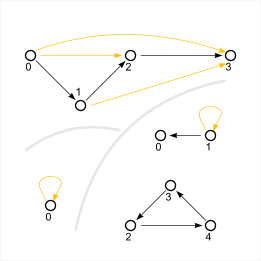
\includegraphics[width=0.5\textwidth]{Abbildungen/Transitivitaet_Graph.png}
                         \caption{Eine transitive Relation als Graph dargestellt.}
                         \label{figure:Mathematik:FormaleGrundlagen:Transitivitaet_Graph}
                    \end{figure}
                    
                \paragraph{Reflexivität}
                    Eine zweistellige Relation $R$ auf einer Menge $M$ ist genau dann reflexiv, wenn $\forall x\colon xRx$ gilt. Wenn kein Element diese Anforderung erfüllt, dass wird die Relation irreflexiv genannt. Der Graph einer reflexiven Funktion ist in Abbildung \ref{figure:Mathematik:FormaleGrundlagen:Reflexivitaet_Graph} dargestellt.
                    
                    Eine reflexive Relation ist zum Beispiel die Kleiner-Gleich-Relation auf den Reellen Zahlen.
                    
                    \begin{figure}
                         \centering
                         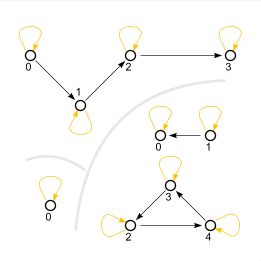
\includegraphics[width=0.5\textwidth]{Abbildungen/Reflexivitaet_Graph.png}
                         \caption{Eine reflexive Relation als Graph dargestellt.}
                         \label{figure:Mathematik:FormaleGrundlagen:Reflexivitaet_Graph}
                    \end{figure}
                    
                \paragraph{Symmetrie}
                    Eine zweistellige Relation $R$ auf einer Menge $M$ ist genau dann symmetrisch, wenn für alle $x, y \in M$ aus $xRy$ stets $yRx$ folgt. Der Graph einer symmetrischen Funktion ist in Abbildung \ref{figure:Mathematik:FormaleGrundlagen:Symmetrie_Graph} dargestellt.
                    
                    Gibt es kein Paar $x, y \in M$ bei dem aus $xRy$ $yRx$ folgt, so nennt man die Relation asymmetrisch.
                    
                    Gibt es nur Paare $x, y \in M$, für die entweder aus $xRy$ nicht $yRx$ folgt oder $x = y$, so nennt man die Relation antisymmetrisch.
                    
                    
                    \begin{figure}
                         \centering
                         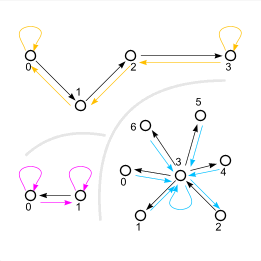
\includegraphics[width=0.5\textwidth]{Abbildungen/Symmetrie_Graph.png}
                         \caption{Eine symmetrische Relation als Graph dargestellt.}
                         \label{figure:Mathematik:FormaleGrundlagen:Symmetrie_Graph}
                    \end{figure}
                    
            \subsubsection{Inversion oder Umkehrung}
                Wenn man eine Relation $r\colon A \rightarrow B$ hat, dann ist die Inversion $r^{-1}\colon B \rightarrow A$. Eine Funktion ist als Relation immer umkehrbar, als Funktion ist sie dagegen genau dann umkehrbar, wenn ihre Umkehrrelation auch wieder eine Funktion ist, also wenn es eine Umkehrfunktion von ihr gibt.                
                    
                    
        \subsection{Funktionen}
            \subsubsection{Eigenschaften}
            % TODO Eigenschaften erläutern
                \begin{itemize}
                    \item Diskret oder Stetig
                    \item Monotonie
                \end{itemize}
                
        
        \subsection{Abschlusseigenschaft}
            Bezüglich der Operation $f: A^n \rightarrow A$ ist eine Menge $M$ mit den Eigenschaften $M \subseteq A$ und $M \not= \emptyset$ abgeschlossen, wenn $\forall a \in M^n\colon f(a) \in M$ gilt.
            
            Die Potenzmenge einer beliebigen Menge $A$ ist abgeschlossen gegenüber der Vereinigung, der Schnittmenge, der Differenzmenge, der symmetrischen Differenzmenge sowie dem Komplement:
            
            \begin{subequations}
                \begin{align}
                    \forall a,b \in P(A^*)&\colon a \cup b \in P(A^*)\\
                    \forall a,b \in P(A^*)&\colon a \cap b \in P(A^*)\\
                    \forall a,b \in P(A^*)&\colon a \setminus b \in P(A^*)\\
                    \forall a,b \in P(A^*)&\colon a \triangle b \in P(A^*)\\
                    \forall a \in P(A^*)&\colon a^C \in P(A^*)\\
                \end{align}
            \end{subequations}
        
    \section[Automatentheorie]{Graphentheorie oder Automatentheorie}
        \subsection{Gerichteter Graph}
            Der Vertex- oder Knotenmenge $S = \{S_0, S_1, S_2, S_3\}$ und der zugehörige Ecken- oder Kantenmenge $R = \{\left(S_0, S_0\right), \left(S_0, S_1\right), \left(S_1, S_2\right), \left(S_2, S_3\right)\}$ kann folgender gerichteter Graph $F\left(S, R\right)$ zugeordnet werden.
            
            \begin{center}
                \begin{tikzpicture}[>=stealth',shorten >=1pt,auto, scale = 1, transform shape, node distance=2 cm]
                    \node[initial,state] (A) {$S_0$};
                    \node[state] (B) [right of=A] {$S_1$};
                    \node[state] (C) [right of=B] {$S_2$};
                    \node[state,accepting] (D) [right of=C] {$S_3$};
                    
                    \path[->] (A) edge [loop above] node [align=center] {} (A)
                              (A) edge []           node [align=center] {} (B)
                              (B) edge []           node [align=center] {} (C)
                              (C) edge []           node [align=center] {} (D);
                \end{tikzpicture}
            \end{center}
            
            Der Graph hat weiterhin folgende Eigenschaften:
            
            \paragraph{Reflexivität}
                Der Knotenpunkt $S_0$ ist reflexive, da es eine Kante von $S_0$ zu $S_0$ gibt.
                
            \paragraph{Transitivität}
                Man kann die Knoten des Graphens in eine Reihenfolge bringen:
                \begin{equation}
                    S_0 \vdash S_0 \vdash S_1 \vdash S_2 \vdash S_3
                \end{equation}
                Da zwei Pfeile aufeinanderfolgen, liegt eine Transitivität oder transitive Hülle vor:
                \begin{equation}
                    S_0 \vdash^* S_2
                \end{equation}
                Ein Spezialfall stellt die transitiv-relative Hülle dar:
                \begin{equation}
                    S_0 \vdash^* S_0
                \end{equation}
                
        \subsection{Kantengewichteter Graph}
            Ein kantengewichteter Graph ist ein Graph mit einer Gewichtungsfunktion $w\colon S \times S \rightarrow \mathbb{R}$.
            
            \begin{center}
                \begin{tikzpicture}[>=stealth',shorten >=1pt,auto,node distance=2 cm, scale = 1, transform shape]
                    \node[initial,state] (A) {$S_0$};
                    \node[state] (B) [right of=A] {$S_1$};
                    \node[state] (C) [right of=B] {$S_2$};
                    \node[state,accepting] (D) [right of=C] {$S_3$};
                    
                    \path[->] (A) edge [loop above] node [align=center] {$30$} (A)
                              (A) edge [above]       node [align=center] {$8$} (B)
                              (B) edge [above]       node [align=center] {$12$} (C)
                              (C) edge [above]       node [align=center] {$13$} (D);
                \end{tikzpicture}
            \end{center}
            
        \subsection[DEA]{Deterministischer endlicher Automat}
            \label{section:DiskreteMathematik:FormaleGrundlagen:DEA}
            Ein deterministischer endlicher Automat ist ein kantengewichteter Graph mit weiteren Eigenschaften.
            
            \subsubsection{Eigenschaften}
                \paragraph{Eingabealphabet}
                    Ein deterministischer endlicher Automat hat eine Eingabealphabet $\Sigma$
                
                \paragraph{Gewichtungsfunktion}
                    Die Gewichtungsfunktion wird als $w\colon S \times S \rightarrow \Sigma$ definiert.
                    
                \paragraph{Zustandsübergangsfunktion}
                    Statt einer Kantenmenge kommt eine Zustandsübergangsfunktion $\delta\colon S \times \Sigma \rightarrow \S$ zum Einsatz.
                    
                    Die Funktion $\delta^*\colon S \times \Sigma^*$ kann ganze Wörter verarbeiten.
                    
                
                    
                \paragraph{Startzustand}
                    Ein Element $S_0 \in S$ wird als Startzustand festgelegt.
                
                \paragraph{Akzeptierende Zustände}
                    Eine Menge $K \subseteq S$ wird als Menge der akzeptierenden Zustände festgelegt.
                    
                \paragraph{Endlich}
                    Das \emph{endlich} in DEA bedeutet, dass sowohl $S$ als auch $\Sigma$ endlich sind:
                    
                    \begin{equation}
                        |S| + |\Sigma| < \infty
                    \end{equation}
                    
        \subsection[NEA]{Nicht deterministischer endlicher Automat}
            Ein nicht deterministischer endlicher Automat unterscheidet sich von einem \hyperref[section:DiskreteMathematik:FormaleGrundlagen:DEA]{DEA} indem seine Zustandsüberführungsfunktion nicht eindeutig ist, sondern eine Menge von Zuständen zurückgibt. Es kann also mehrere Zustände für ein gegebenes Wort geben.
            Formal wird ein NEA durch ein Quintupel aus den Elementen $(S, \Sigma, \delta, S_0, K)$ definiert:
            
            \paragraph{Zustände ($S$)} Eine endliche, nicht leere Menge von möglichen Zuständen des DEA.
            
            \paragraph{Eingabealphabet ($\Sigma$)} Eine endliche, nicht leere Menge aller Buchstaben die die Zustandsübergangsfunktion akzeptiert.
            
            \paragraph{Zustandsübergangsfunktion ($\delta$)} Die Übergangsrelation gibt für einen gegebenen Zustand $s \in S$ und ein Buchstaben $a \in \Sigma$ die Menge der neuen Zustände zurück. Formal wird dies wie folgt geschrieben:
            	\begin{equation}
            	    \delta: s \times a \rightarrow S^*
            	\end{equation}
            	
        	\paragraph{Startzustand ($S_0$)}
                Ein Element $S_0 \in S$ wird als Startzustand festgelegt.
                
    	\paragraph{Akzeptierende Zustände ($K$)}
    	    Eine Menge $K \subseteq S$ wird als Menge der akzeptierenden Zustände festgelegt.
    	    
                    
        \subsection{Chomsky-Hierarchie}
            Die Chomsky-Hierarchie ordnet alle Sprachen mit 4 Typen:
            
            \paragraph{Alle Sprachen}
                Die Potenzmenge des Alphabetes $P(\Sigma^*)$ ist die überabzählbare Menge aller Sprachen.
            
            \paragraph{Typ 0}
                Type 0 Sprachen sind Phrasenstrukturen und stellen die Menge aller berechenbarer Probleme dar. Typ 0 Sprachen sind eine Teilmenge aller Sprachen
                
            \paragraph{Typ 1}
                Typ 1 Sprachen sind kontextsensitive Sprachen und sind eine Teilmenge der Typ 0 Sprachen.
                
            \paragraph{Typ 2}
                Typ 2 Sprachen sind kontextfreie Sprachen und sind eine Teilmenge der Typ 1 Sprachen.
                
            \paragraph{Typ 3}
                Typ 3 Sprachen sind reguläre Sprachen mit einer regulären Grammatik und sind eine Teilmenge der Typ 2 Sprachen. Sie werden von endlichen Automaten akzeptiert.
\end{document}
